\subsection*{Motivation}

Consider as motivation the Motorcycle Accident Dataset
\cite{silv:1985}.  It is a classic data set used in recent literature
\cite{rasm:ghah:nips:2002} to demonstrate the success of nonstationary
regression models.  The data consists of measurements of the
acceleration of the head of a motorcycle rider as a function of time
in the first moments after an impact.  Many authors have commented on
the existence of two---perhaps three---regimes in the data over time
where the characteristics of the mean process and noise level change
(i.e., a nonstationarity and heteroskedasticity, respectively).  It
can be interesting to see how various candidate models handle this
nuance.

\begin{figure}[ht!]
\centering
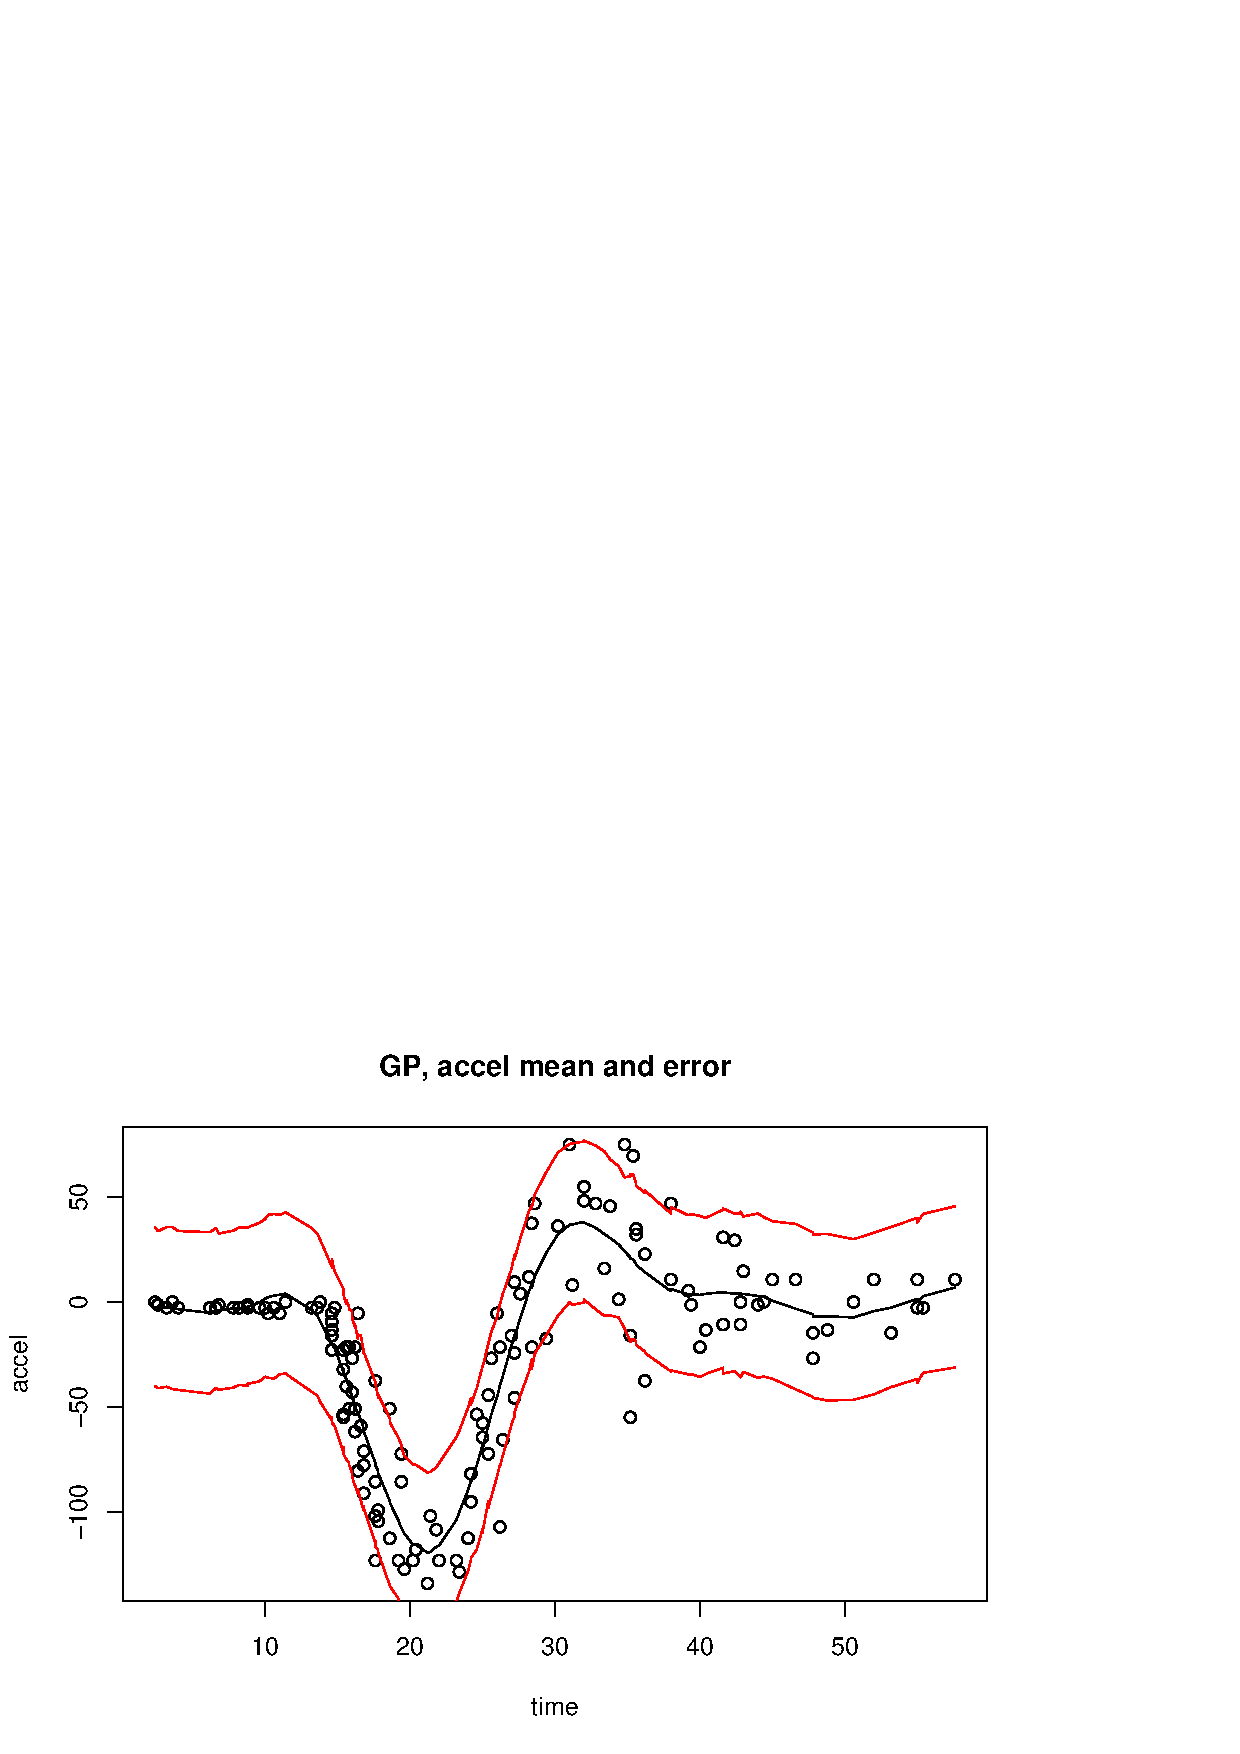
\includegraphics[trim=0 25 0 0]{motovate_bgp}
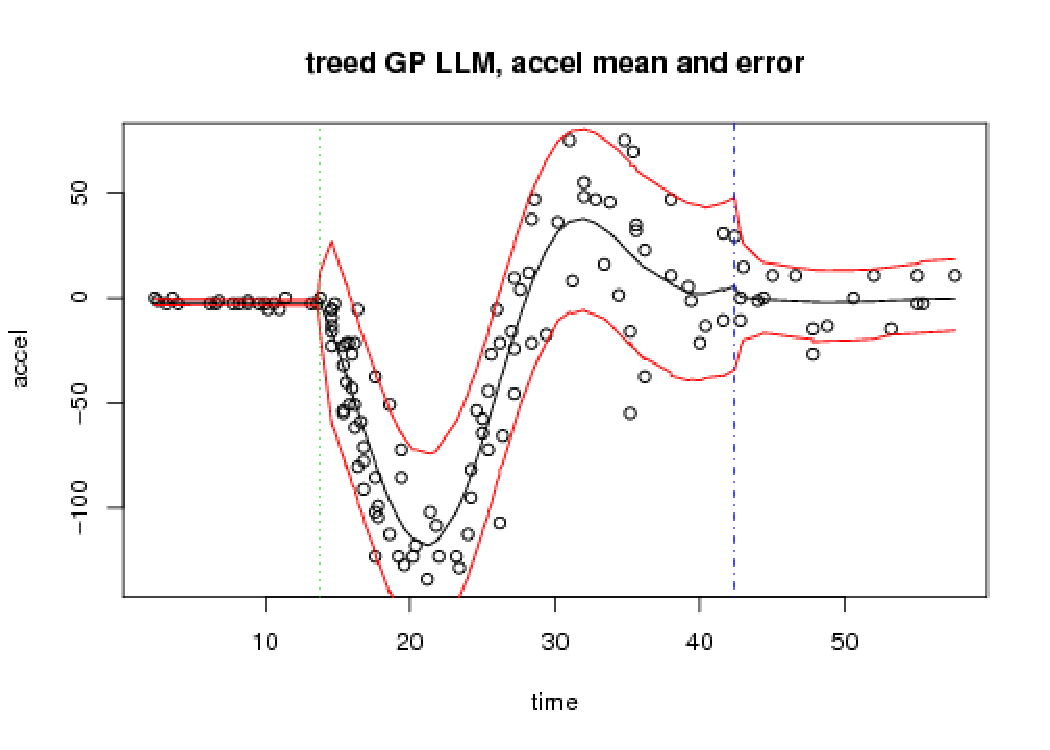
\includegraphics[trim=0 25 0 0]{motovate_btgp}
\caption{Fit of the Motorcycle Accident Dataset using a GP ({\em top})
  and treed GP model ({\em bottom}).  The $x$-axis is time in
  milliseconds after an impact; the $y$--axis is acceleration of the
  helmet of a motorcycle rider measured in ``$g$'s'' in a simulated
  impact.}
\label{f:motivate}
\end{figure}

Figure \ref{f:motivate} shows a fit of this data using a standard
(stationary) Gaussian process (GP; {\em left}), and the treed GP model
({\em right}).\footnote{Note that these plots are {\em static}, i.e.,
  they were not generated in--line with {\tt R} code.  See Section
  \ref{sec:moto} for {\em dynamic} versions.}  Notice how stationary
GP model is unable to capture the smoothness in the linear section(s),
nor the decreased noise level.  We say that the standard GP model is
stationary because it has a single fixed parameterization throughout
the input space.  An additive model would be inappropriate for similar
reasons.  In contrast, the treed GP model is able to model the first
linear part, the noisy ``whiplash'' middle section, and the smooth
(possibly linear) final part with higher noise level, thus exhibiting
nonstationary modeling behavior and demonstrating an ability to cope
with heteroskedasticity.

The remainder of this paper describes the treed GP model in detail,
and provides illustrations though example.  There are many special
cases of the treed GP model, e.g., the linear model (LM), treed LM,
stationary GP, etc.. These are outlined and demonstrated as well.


%%% Local Variables: 
%%% mode: latex
%%% TeX-master: "tgp"
%%% End: 
